\documentclass[12pt,a4paper]{article}
\usepackage[utf8]{inputenc}
\usepackage[spanish,es-tabla]{babel}
\usepackage{geometry}
\usepackage{graphicx}
\usepackage{multirow}
\usepackage{tabularx}
\usepackage{longtable}
\usepackage{float}
\usepackage{amsmath}
\usepackage{amssymb}
\usepackage{mathptmx}
\usepackage{fancyhdr}
\usepackage{array}
\usepackage[table]{xcolor}
\usepackage{titlesec}
\usepackage{setspace}
\usepackage{microtype}
\usepackage{lastpage}
\usepackage{booktabs}
\usepackage{enumitem}
\usepackage{hyperref}

\hypersetup{
    colorlinks=true,
    linkcolor=black,
    citecolor=blue!70!black,
    urlcolor=blue!70!black
}

\graphicspath{{images/}{../images/}{./}}

\geometry{
    top=4.7cm,
    bottom=2.5cm,
    left=2.5cm,
    right=2.5cm,
    headheight=3.9cm,
    headsep=0.4cm
}

\setstretch{1.15}
\setlength{\parindent}{0pt}
\setlength{\parskip}{0.45em}
\setlength{\tabcolsep}{4pt}

\titleformat{\section}
  {\normalfont\fontsize{12}{14.5}\bfseries}{\thesection.}{0.6em}{\uppercase}
\titlespacing*{\section}
  {0pt}{1.8ex plus 0.4ex minus 0.2ex}{0.6ex plus 0.2ex}

\titleformat{\subsection}
  {\normalfont\fontsize{11.5}{13.5}\bfseries}{\thesubsection.}{0.5em}{}
\titlespacing*{\subsection}
  {0pt}{1.4ex plus 0.3ex minus 0.1ex}{0.4ex plus 0.1ex}

\titleformat{\subsubsection}
  {\normalfont\fontsize{10.5}{12.5}\bfseries\itshape}{\thesubsubsection.}{0.4em}{}
\titlespacing*{\subsubsection}
  {0pt}{1.1ex plus 0.2ex minus 0.1ex}{0.3ex plus 0.1ex}

\newcolumntype{Y}{>{\centering\arraybackslash}X}
\newcolumntype{L}{>{\raggedright\arraybackslash}X}
\newcolumntype{C}{>{\centering\arraybackslash}X}
\newcolumntype{R}{>{\raggedleft\arraybackslash}X}

\definecolor{headerred}{RGB}{180, 0, 0}
\definecolor{darkred}{RGB}{140, 0, 0}
\definecolor{lightgraybg}{RGB}{248, 248, 248}
\definecolor{tableheader}{RGB}{232, 238, 246}
\definecolor{navyheader}{RGB}{0, 52, 94}

\newcommand{\docCodigo}{TI-SIGE-ENT-F1-009}
\newcommand{\docVersion}{2.0}
\newcommand{\docProceso}{INGENIERÍA DE SOFTWARE / GESTIÓN DE PROYECTOS}
\newcommand{\docElaboracion}{07/10/2026}
\newcommand{\docTitulo}{NORMAS Y ESTÁNDARES EN PROYECTOS}
\newcommand{\docRevision}{12/10/2026}

\newcommand{\encabezadofrecuente}{%
    \renewcommand{\arraystretch}{1.15}%
    \noindent\makebox[\textwidth][c]{%
    \begin{tabularx}{\textwidth}{|>{\centering\arraybackslash}m{2.8cm}|Y|>{\centering\arraybackslash}m{4.8cm}|}
        \hline
        \multirow{4}{2.8cm}{\centering\raisebox{-1.15cm}{
\includegraphics[width=2.5cm,height=2.0cm,keepaspectratio]{images/logo.png}}}
        & \textbf{\fontsize{9.5}{11.5}\selectfont SHINAX} 
        & \textbf{\fontsize{8}{10}\selectfont CÓDIGO:} \fontsize{8}{10}\selectfont \docCodigo \\
        \cline{3-3}
        & \textbf{\fontsize{8.5}{10.5}\selectfont SOFTWARE STUDIO} 
        & \textbf{\fontsize{8}{10}\selectfont VERSIÓN:} \fontsize{8}{10}\selectfont \docVersion \\
        \cline{2-3}
        & \textbf{\fontsize{8}{10}\selectfont PROCESO:} \fontsize{8}{10}\selectfont \docProceso 
        & \textbf{\fontsize{8}{10}\selectfont ELABORACIÓN:} \fontsize{8}{10}\selectfont \docElaboracion \\
        \cline{2-3}
        & \textbf{\fontsize{9}{11}\selectfont \docTitulo} 
        & \textbf{\fontsize{8}{10}\selectfont ÚLTIMA REVISIÓN:} \fontsize{8}{10}\selectfont \docRevision \\
        \hline
    \end{tabularx}%
    }%
}

\pagestyle{fancy}
\fancyhf{}
\fancyhead[C]{\encabezadofrecuente}
\fancyfoot[C]{\fontsize{10}{12}\selectfont Página \thepage\ de \pageref{LastPage}}
\renewcommand{\headrulewidth}{0pt}

\begin{document}

% =============================================================
% 1. TÍTULO
% =============================================================
\noindent{\fontsize{10.5}{12.5}\selectfont \textbf{Integrantes:} Heidi Villavicencio \quad$\vert$\quad Steeven Toala \quad$\vert$\quad Nixon Hurtado \quad$\vert$\quad Andrea Vásquez}

\vspace{0.25cm}
\section{Título}
\textbf{Denominación del Entregable:} Informe Técnico de Aplicación de Normas y Estándares en el Proyecto SIGE (Sistema Web para la Gestión, Seguimiento y Aprobación de Informes y Planes de Trabajo de la FISEI - UTA).



% =============================================================
% 2. INTRODUCCIÓN
% =============================================================
\section{Introducción}
El desarrollo del proyecto SIGE surge ante la necesidad de digitalizar y optimizar el proceso de elaboración, seguimiento, revisión y aprobación de los Planes de Trabajo Docente y los Informes Semestrales de Cumplimiento en la FISEI de la Universidad Técnica de Ambato. Históricamente, estos procedimientos se gestionaban mediante documentos físicos y hojas de cálculo dispersas, lo cual provocaba demoras administrativas, inconsistencias en el cálculo de horas reglamentarias y dificultades para custodiar las evidencias académicas exigidas por el Sistema de Gestión de la Calidad (SGC) institucional.

Para asegurar que la plataforma desarrollada cumpla con criterios de ingeniería rigurosos, este informe presenta la aplicación práctica de normas y estándares internacionales a lo largo del ciclo de vida del proyecto. Se prioriza un conjunto núcleo de estándares reconocidos en la ingeniería de software y la gestión de proyectos: ISO/IEC 25010 para la calidad del producto, ISO/IEC/IEEE 29148 para la ingeniería de requisitos, ISO/IEC/IEEE 12207 para los procesos del ciclo de vida, ISO/IEC 27001 para la seguridad de la información, IEEE 828 para la gestión de la configuración, ISO 31000 para la gestión de riesgos y la guía PMBOK del PMI para la dirección del proyecto.

Asimismo, se incorporan prácticas de apoyo y guías técnicas como OWASP Top 10 para la seguridad web y marcos ágiles (Scrum y Kanban) para la organización operativa de tareas. A diferencia de un texto teórico, el presente documento fundamenta cada estándar a partir de su implementación real en el sistema SIGE, detallando qué establece la norma, cómo se aplica en la plataforma, qué ejemplo concreto de código o configuración la sustenta y qué evidencia técnica respalda su ejecución.

% =============================================================
% 3. OBJETIVO
% =============================================================
\section{Objetivo}

\subsection{Objetivo General}
Documentar y justificar la aplicación práctica de las normas y estándares internacionales de ingeniería de software y gestión de proyectos en el sistema SIGE, evidenciando su implementación técnica mediante ejemplos concretos en los módulos de requisitos, arquitectura, desarrollo, seguridad, configuración y pruebas.

\subsection{Objetivos Específicos}
\begin{itemize}[leftmargin=1.5em, itemsep=2pt]
    \item Identificar y jerarquizar las normas técnicas aplicables al proyecto, distinguiendo los estándares internacionales formales de las guías técnicas y prácticas de desarrollo complementarias.
    \item Describir la aplicación concreta de cada norma en el sistema SIGE mediante la estructura: qué establece, aplicación en SIGE, ejemplo técnico y evidencia verificable.
    \item Vincular cada una de las 44 actividades y 7 hitos de la Estructura de Desglose del Trabajo (EDT) con su norma o referencia rectora y su medio de verificación en el repositorio.
    \item Definir las políticas técnicas y de calidad que el equipo estudiantil implementa para garantizar la consistencia de los datos, la seguridad de las evidencias y la mantenibilidad del código.
\end{itemize}

% =============================================================
% 4. ALCANCE
% =============================================================
\section{Alcance}

\subsection{Alcance Incluido}
\begin{itemize}[leftmargin=1.5em, itemsep=2pt]
    \item Aplicación de normas y estándares en las 5 fases del proyecto SIGE: Fase 1 (Análisis y Planificación), Fase 2 (Diseño Rápido y Arquitectura), Fase 3 (Desarrollo Iterativo Core), Fase 4 (Pruebas QA, Seguridad e Integración) y Fase 5 (Despliegue, Documentación y Cierre).
    \item Cobertura de las 7 normas núcleo del proyecto: ISO/IEC 25010:2023, ISO/IEC/IEEE 29148:2018, ISO/IEC/IEEE 12207:2017, ISO/IEC 27001:2022, IEEE Std 828-2012, ISO 31000:2018 y PMI PMBOK 7ma Edición.
    \item Incorporación de guías técnicas y operativas de apoyo: OWASP Top 10 (2021) para seguridad de endpoints, Scrum y Kanban para la gestión del flujo de trabajo, e ISO 32000-1 e ISO/IEC 29500 para la exportación de documentos oficiales en formatos PDF y Word.
    \item Trazabilidad completa sobre los componentes del repositorio del proyecto SIGE: base de datos relacional PostgreSQL, API REST en Node.js Express, frontend interactivo en React 19 y almacenamiento de objetos MinIO S3 en contenedores Docker.
\end{itemize}

\subsection{Exclusiones}
\begin{itemize}[leftmargin=1.5em, itemsep=2pt]
    \item Certificaciones institucionales formales de tercera parte (auditorías externas oficiales de acreditación ISO o CMMI), dado que el alcance corresponde a un proyecto académico de titulación y cátedra universitaria.
    \item Evaluación de procesos corporativos de recursos humanos bajo ISO 30414 o niveles de madurez organizacional CMMI, por no resultar pertinentes ni proporcionados para un equipo de cuatro desarrolladores universitarios.
    \item Modificación del marco regulatorio legal y reglamentos vigentes de la Universidad Técnica de Ambato.
\end{itemize}

% =============================================================
% 5. DEFINICIONES
% =============================================================
\section{Definiciones}
\begin{itemize}[leftmargin=1.5em, itemsep=2pt]
    \item \textbf{ISO (International Organization for Standardization):} Federación mundial de organismos nacionales de normalización que elabora normas técnicas internacionales voluntarias para asegurar calidad, seguridad y eficiencia.
    \item \textbf{IEC (International Electrotechnical Commission):} Organización líder mundial en la preparación y publicación de normas internacionales para todas las tecnologías eléctricas, electrónicas y tecnologías afines.
    \item \textbf{IEEE (Institute of Electrical and Electronics Engineers):} Organización técnica profesional dedicada al avance de la tecnología, editora de estándares reconocidos para ingeniería de software y hardware.
    \item \textbf{PMI (Project Management Institute):} Asociación profesional líder en dirección de proyectos, creadora del estándar PMBOK (Guía de los Fundamentos para la Dirección de Proyectos).
    \item \textbf{SGC (Sistema de Gestión de la Calidad):} Conjunto de políticas, procesos y procedimientos formalizados en la Universidad Técnica de Ambato para planificar, ejecutar y evaluar las actividades académicas.
    \item \textbf{Validation Gate (Compuerta de Validación):} Mecanismo lógico implementado en el backend del software que verifica el cumplimiento estricto de reglas de negocio antes de permitir la transición de estado de un documento.
    \item \textbf{URL Prefirmada (Presigned URL):} Enlace temporal con firma criptográfica que otorga acceso controlado de lectura o escritura a un objeto almacenado en MinIO S3 durante un período de tiempo predefinido sin exponer credenciales del servidor.
    \item \textbf{EDT / WBS (Estructura de Desglose del Trabajo):} Descomposición jerárquica del alcance total del proyecto orientada a entregables medibles, facilitando la planificación, asignación y control del trabajo.
    \item \textbf{Línea Base de Configuración:} Conjunto de especificaciones y elementos de código formalmente aprobados en un punto específico del tiempo (como el congelamiento de código o Code Freeze), que solo puede modificarse mediante un procedimiento controlado de cambios.
    \item \textbf{JWT (JSON Web Token):} Estándar abierto (RFC 7519) para la transmisión segura de afirmaciones de identidad entre dos partes mediante tokens compactos y firmados digitalmente.
\end{itemize}

% =============================================================
% 6. RESPONSABILIDADES
% =============================================================
\section{Responsabilidades}

La distribución de responsabilidades en el equipo de desarrollo para la aplicación y verificación de normas y estándares en el proyecto SIGE se organiza formalmente de la siguiente manera:

\begin{itemize}[leftmargin=1.5em, itemsep=2pt]
    \item \textbf{Steeven Toala (Líder de Proyecto / Arquitecto de Software):}
    Responsable de la dirección del proyecto bajo los principios de PMBOK, definición de la arquitectura técnica (ISO/IEC/IEEE 42010), orquestación de contenedores en Docker (ISO/IEC 25010 en portabilidad), configuración del repositorio y políticas de ramas Git (IEEE 828), y aseguramiento de la infraestructura de red interna (ISO/IEC 27001).
    \item \textbf{Heidi Villavicencio (Analista de Requisitos / Diseñadora UI-UX):}
    Responsable de la captura, análisis y documentación de los 24 requisitos funcionales y 10 no funcionales bajo la norma ISO/IEC/IEEE 29148 y la plantilla IEEE 830, elaboración de diagramas de casos de uso (UML), diseño de la experiencia de usuario y accesibilidad en Figma (ISO 9241-210), y redacción de manuales operativos de usuario (ISO/IEC/IEEE 26514).
    \item \textbf{Nixon Hurtado (Desarrollador Backend / DBA):}
    Responsable del modelado y persistencia relacional en PostgreSQL bajo ISO/IEC 9075 (SQL), implementación de controladores y Validation Gates en Express (ISO/IEC 25010 en adecuación funcional), mecanismos de mitigación de inyección y autenticación segura bajo directrices OWASP Top 10, y servicio de almacenamiento en MinIO S3 con URLs prefirmadas (ISO/IEC 27001).
    \item \textbf{Andrea Vasquez (Desarrolladora Frontend / QA Tester):}
    Responsable del desarrollo de componentes modulares en React 19 bajo buenas prácticas de ingeniería de software, implementación del Wizard modular y la Matriz interactiva de actividades, diseño y ejecución de casos de prueba funcional de extremo a extremo (ISO/IEC/IEEE 29119), y seguimiento de tareas en el tablero del proyecto.
    \item \textbf{Ing. Paulo Torres, Mg. (Docente Evaluador y Tutor Metodológico):}
    Responsable del seguimiento académico, revisión técnica periódica de los entregables de cada fase, validación de la correspondencia entre actividades y estándares internacionales, y evaluación formativa del proyecto.
\end{itemize}

% =============================================================
% 7. NORMATIVA LEGAL Y TÉCNICA
% =============================================================
\section{Normativa Legal y Técnica}

\subsection{Marco Legal Institucional y Nacional}
\begin{itemize}[leftmargin=1.5em, itemsep=2pt]
    \item \textbf{Ley Orgánica de Educación Superior (LOES):} Normativa nacional que rige a las universidades del Ecuador, exigiendo calidad académica, rendición de cuentas sobre la carga laboral docente y preservación de evidencias documentales de las actividades universitarias.
    \item \textbf{Reglamento de Carrera y Escalafón del Profesor e Investigador del CES:} Marco regulatorio emitido por el Consejo de Educación Superior que establece la distribución de horas de docencia, investigación, vinculación y gestión académica institucional.
    \item \textbf{Reglamento y Procedimientos del SGC de la UTA:} Formatos oficiales institucionales vigentes UTA-SGC-A-2-1-P7-T1 (Plan de Trabajo Docente) y UTA-SGC-A-2-1-P7-T2 (Informe Semestral de Actividades Docentes), cuyos campos y fórmulas son replicados en el sistema SIGE.
\end{itemize}

\subsection{Marco Técnico Internacional}
El proyecto organiza sus referencias técnicas en dos niveles claramente diferenciados para evitar confusión entre estándares formales y guías operativas:

\textbf{A. Normas Principales (Núcleo Formal del Proyecto):}
\begin{itemize}[leftmargin=1.5em, itemsep=2pt]
    \item \textbf{ISO/IEC 25010:2023:} Calidad del producto de software y características de calidad en uso (SQuaRE).
    \item \textbf{ISO/IEC/IEEE 29148:2018:} Ingeniería de requisitos en el ciclo de vida del software.
    \item \textbf{ISO/IEC/IEEE 12207:2017:} Procesos del ciclo de vida del software.
    \item \textbf{ISO/IEC 27001:2022:} Gestión de la seguridad de la información y controles de seguridad.
    \item \textbf{IEEE Std 828-2012:} Gestión de la configuración en sistemas y software (SCM).
    \item \textbf{ISO 31000:2018:} Directrices para la gestión del riesgo.
    \item \textbf{PMI PMBOK (7ma Edición):} Principios y dominios de desempeño para la dirección de proyectos.
\end{itemize}

\textbf{B. Guías Técnicas y Prácticas Complementarias de Apoyo:}
\begin{itemize}[leftmargin=1.5em, itemsep=2pt]
    \item \textbf{OWASP Top 10 (Edición 2021):} Guía de seguridad de aplicaciones web para la prevención de fallos comunes (inyección, control de acceso roto, fallas criptográficas).
    \item \textbf{Prácticas Ágiles (Scrum y Kanban):} Técnicas de trabajo colaborativo para la división de tareas en iteraciones y el seguimiento visual del flujo en tableros Kanban.
    \item \textbf{IEEE Std 830-1998:} Práctica recomendada para la especificación de requisitos de software (SRS) [se utiliza como plantilla de redacción subordinada a ISO 29148].
    \item \textbf{ISO 32000-1 e ISO/IEC 29500:} Estándares de formatos abiertos para documentos PDF y DOCX OpenXML, aplicados en la exportación oficial de planes e informes.
\end{itemize}

% =============================================================
% 8. MÉTODO, POLÍTICAS Y CONTENIDOS
% =============================================================
\section{Método, Políticas y Contenidos}

\subsection{Enfoque Metodológico y Criterios de Selección}
Para garantizar que la adopción de estándares agregue valor real y no represente una carga burocrática vacía, el equipo estableció los siguientes criterios metodológicos de selección:

\begin{enumerate}[leftmargin=1.5em, itemsep=2pt]
    \item \textbf{Pertinencia al Contexto Universitario:} Cada estándar seleccionado responde a un problema tangible del proyecto. Por ejemplo, se seleccionó ISO/IEC 27001 porque el sistema gestiona evidencias docentes sensibles (oficios y actas) que requieren confidencialidad e integridad, no por acumular menciones teóricas.
    \item \textbf{Separación entre Procesos del Negocio y Calidad del Software:} Se clarifica que la norma ISO 9001 rige el Sistema de Gestión de la Calidad de la Universidad Técnica de Ambato y sus procedimientos documentados. El software SIGE no certifica a la universidad en ISO 9001; lo que hace es automatizar dichos procedimientos institucionales aplicando internamente el estándar ISO/IEC 25010 para garantizar la calidad del producto software.
    \item \textbf{Adopción Proporcional de Marcos de Gestión:} El proyecto aplica los principios del PMBOK para la planificación estructurada del alcance (EDT), cronograma e hitos de entrega, combinándolos con la agilidad de Scrum y Kanban para la asignación semanal de tareas entre los cuatro desarrolladores.
\end{enumerate}

\subsection{Políticas Técnicas Adoptadas en el Proyecto SIGE}
El equipo formalizó cuatro políticas operativas de cumplimiento obligatorio durante el desarrollo:

\begin{enumerate}[leftmargin=1.5em, itemsep=2pt]
    \item \textbf{Política de Control de Configuración y Ramas Git (IEEE 828):} Ningún cambio se introduce directamente en la rama principal (\texttt{main}). Las nuevas funcionalidades se desarrollan en ramas secundarias de tipo \texttt{feature/*}, se integran en \texttt{develop} mediante revisión de código entre compañeros y se congelan en una versión Release Candidate antes de las pruebas formales.
    \item \textbf{Política de Validación Estricta de Negocio (Validation Gates):} Queda prohibido el paso de un plan o informe al estado de revisión si no satisface la totalidad de las reglas institucionales: sumatoria obligatoria de 160 horas por período y justificación respaldada con medios de verificación en cada actividad.
    \item \textbf{Política de Seguridad y Custodia de Evidencias (ISO 27001 y OWASP):} Los archivos cargados no se almacenan en el sistema de archivos del servidor web ni se exponen de forma pública. Se custodian en un servicio de objetos MinIO S3 y solo se accede a ellos mediante URLs temporales prefirmadas de 15 minutos de vigencia generadas por el backend tras validar la sesión del usuario.
    \item \textbf{Política de Gestión Preventiva de Riesgos (ISO 31000):} Toda operación crítica sobre la base de datos que involucre múltiples tablas (por ejemplo, guardar la matriz de actividades junto con sus metas y ponderaciones) debe ejecutarse dentro de una transacción atómica de PostgreSQL, asegurando que ante cualquier error se realice un \texttt{ROLLBACK} automático que evite la corrupción de los registros.
\end{enumerate}

\subsection{Análisis de Pertinencia y Exclusión de Marcos No Aplicables}
Con el objetivo de mantener la veracidad técnica del informe, se justifican las siguientes exclusiones:
\begin{itemize}[leftmargin=1.5em, itemsep=2pt]
    \item \textbf{Exclusión de CMMI (Capability Maturity Model Integration):} CMMI evalúa la madurez de procesos en empresas y organizaciones medianas a grandes con proyectos a largo plazo y auditorías formales de valoración. Declarar cumplimiento de CMMI en un proyecto académico de 80 días con un equipo de cuatro estudiantes resultaría desproporcionado e irreal. Por tanto, se utiliza formalmente la norma ISO/IEC/IEEE 12207 para estructurar el ciclo de vida.
    \item \textbf{Exclusión de ISO 30414 (Métricas de Capital Humano):} Esta norma define directrices de reporte de recursos humanos corporativos para organizaciones con áreas formales de talento humano. En SIGE, la coordinación del equipo se gestiona mediante la distribución de roles y la matriz RACI del PMBOK, descartando ISO 30414.
\end{itemize}

% =============================================================
% 9. DESCRIPCIÓN DE ACTIVIDADES Y APLICACIÓN DE NORMAS
% =============================================================
\section{Descripción de actividades}

Esta sección constituye el núcleo del presente informe técnico. A continuación se desglosa la aplicación de cada norma y estándar seleccionado mediante la estructura: qué establece, aplicación en SIGE, ejemplo concreto y evidencia verificable, seguido de la matriz de correspondencia con la Estructura de Desglose del Trabajo (EDT).

\subsection{Aplicación Detallada de las Normas Principales (Núcleo del Proyecto)}

% --- 1. ISO 25010 ---
\subsubsection{Norma: ISO/IEC 25010:2023 -- Calidad del Producto de Software}

\textbf{Qué establece:}
La norma ISO/IEC 25010 (perteneciente a la familia SQuaRE) describe un modelo integral para evaluar la calidad del producto de software a través de características bien definidas: adecuación funcional, eficiencia de desempeño, compatibilidad, usabilidad, fiabilidad, seguridad, mantenibilidad y portabilidad. Permite asegurar que el software no solo funcione, sino que opere de forma confiable, intuitiva y reproducible en distintos entornos.

\textbf{Aplicación en SIGE:}
En el proyecto SIGE, esta norma se aplica directamente en cuatro características prioritarias:
\begin{itemize}[leftmargin=1.5em, itemsep=2pt]
    \item \textbf{Adecuación Funcional:} Los formularios y módulos digitales reproducen al 100\% los requerimientos de los formatos institucionales UTA-SGC-A-2-1-P7-T1 y T2, impidiendo estados inconsistentes mediante validaciones de reglas de negocio en el backend.
    \item \textbf{Portabilidad:} La aplicación completa se empaqueta en contenedores Docker, garantizando que el sistema opere de forma idéntica en el entorno de desarrollo local de cada integrante y en el servidor de despliegue.
    \item \textbf{Fiabilidad y Tolerancia a Fallos:} El editor de texto enriquecido de planes e informes implementa un mecanismo de autoguardado asíncrono con temporizador de inactividad (\texttt{debounce}), evitando que el docente pierda información redactada en caso de corte de energía o cierre accidental de pestaña.
    \item \textbf{Usabilidad:} Se construyó una interfaz basada en un asistente secuencial por pestañas (Datos Informativos, Justificación, Matriz de Actividades y Firmas) que guía paso a paso al docente reduciendo la tasa de errores de ingreso.
\end{itemize}

\textbf{Ejemplo en SIGE:}
En el servicio de validación de planes del backend, cuando un usuario intenta cambiar el estado de su plan a \texttt{ENVIADO\_REVISION}, el sistema ejecuta la verificación de horas:
\begin{quote}
Si la sumatoria de las horas asignadas en la matriz de actividades no suma exactamente 160 horas (exigencia reglamentaria de la FISEI), el backend rechaza la petición con código HTTP 400 y devuelve un mensaje indicando el número exacto de horas faltantes o excedentes. Esto garantiza que ningún plan con errores aritméticos llegue a la bandeja del Coordinador de Carrera.
\end{quote}

\textbf{Evidencia:}
Configuración de contenedores de desarrollo y producción, módulo de edición guiada en el frontend, servicio de validación en el controlador de planes y pruebas de adecuación funcional de la Fase 4.

% --- 2. ISO 29148 ---
\subsubsection{Norma: ISO/IEC/IEEE 29148:2018 -- Ingeniería de Requisitos}

\textbf{Qué establece:}
El estándar ISO/IEC/IEEE 29148 define los procesos y recomendaciones para la ingeniería de requisitos a lo largo del ciclo de vida del software. Establece lineamientos para la obtención, análisis, especificación, verificación y validación de requerimientos, exigiendo que cada requisito sea necesario, no ambiguo, consistente, trazable y verificable.

\textbf{Aplicación en SIGE:}
Durante la Fase 1 del proyecto se aplicó este estándar para estructurar la Especificación de Requisitos de Software (SRS). Se relevaron formalmente las necesidades de los tres roles principales del sistema (Docente Elaborador, Coordinador Revisor y Subdecano Validador), clasificando el alcance en 24 requisitos funcionales (RF-01 a RF-24) y 10 requisitos no funcionales (RNF-01 a RNF-10). Cada requisito se formuló con identificador único, descripción precisa, criterios de aceptación y relación de dependencia.

\textbf{Ejemplo en SIGE:}
El requisito funcional RF-05 se redactó siguiendo las directrices de no ambigüedad y verificabilidad de ISO 29148:
\begin{quote}
\textbf{RF-05 (Validación Aritmética de Carga Horaria):} El sistema debe calcular automáticamente la suma de horas de las actividades distribuidas en docencia, tutorías, investigación y gestión, exigiendo que la sumatoria total sea idéntica a 160 horas semestrales antes de habilitar el botón de envío para revisión. \\
\textbf{Criterio de Aceptación:} Si el total es menor a 160 horas, se muestra una alerta en color ámbar con el saldo restante; si es mayor a 160 horas, se muestra una alerta en color rojo indicando el exceso. Solo cuando el contador es exactamente 160, el botón de envío pasa a estado activo.
\end{quote}

\textbf{Evidencia:}
Documento formal de Especificación de Requisitos de Software (SRS) y matriz de trazabilidad de requisitos entre la EDT y el código fuente.

% --- 3. ISO 12207 ---
\subsubsection{Norma: ISO/IEC/IEEE 12207:2017 -- Procesos del Ciclo de Vida del Software}

\textbf{Qué establece:}
Esta norma internacional proporciona un marco común de procesos para el ciclo de vida del software, cubriendo desde la concepción del sistema hasta su retiro. Define procesos primarios (adquisición, desarrollo, operación y mantenimiento), procesos de soporte (documentación, gestión de configuración, aseguramiento de calidad, verificación y validación) y procesos organizacionales.

\textbf{Aplicación en SIGE:}
El proyecto adaptó los procesos técnicos de ISO 12207 para estructurar el desarrollo en cinco fases secuenciales con hitos de control formal:
\begin{enumerate}[leftmargin=1.5em, itemsep=2pt]
    \item \textbf{Fase 1 (Análisis y Planificación):} Procesos de definición de requisitos y gobernanza inicial (Hito 1).
    \item \textbf{Fase 2 (Diseño Rápido y Arquitectura):} Procesos de diseño arquitectónico y de datos (Hito 2).
    \item \textbf{Fase 3 (Desarrollo Iterativo Core):} Procesos de construcción e integración modular de software (Hitos 3, 4 y 5).
    \item \textbf{Fase 4 (Pruebas QA, Seguridad e Integración):} Procesos formales de verificación, validación y corrección (Hito 6).
    \item \textbf{Fase 5 (Despliegue, Capacitación y Cierre):} Procesos de transición a producción y entrega de la solución (Hito 7).
\end{enumerate}

\textbf{Ejemplo en SIGE:}
Al culminar la Fase 2, se aplicó la compuerta de salida del proceso de diseño: no se inició la codificación de la Fase 3 hasta que los diagramas de arquitectura en capas, el modelo entidad-relación en PostgreSQL y los prototipos de Figma contaron con la revisión y visto bueno del docente tutor en el Hito 2. Esto previno costosas reestructuraciones de la base de datos en fases avanzadas.

\textbf{Evidencia:}
Estructura de Desglose del Trabajo (EDT) del proyecto, cronograma maestro de actividades en Microsoft Project y actas de aprobación semanal de hitos institucionales.

% --- 4. ISO 27001 ---
\subsubsection{Norma: ISO/IEC 27001:2022 -- Gestión de la Seguridad de la Información}

\textbf{Qué establece:}
La norma ISO/IEC 27001 establece los requisitos para planificar, implementar, mantener y mejorar un Sistema de Gestión de Seguridad de la Información (SGSI). Se enfoca en proteger la confidencialidad, integridad y disponibilidad de los activos de información mediante la aplicación de controles de seguridad técnicos, organizacionales y físicos.

\textbf{Aplicación en SIGE:}
En SIGE se gestionan activos de información institucional sensibles: informes de desempeño de docentes, justificaciones de actividades y documentos PDF adjuntos como evidencias probatorias (oficios, actas de notas, certificados). Se implementaron tres controles de seguridad inspirados en el Anexo A de la norma:
\begin{itemize}[leftmargin=1.5em, itemsep=2pt]
    \item \textbf{Control A.5.15 (Control de Accesos):} Implementación de control de acceso basado en roles (RBAC). Un docente solo puede consultar y editar sus propios borradores; un coordinador solo puede revisar expedientes de su carrera; y únicamente el subdecano puede emitir la resolución final.
    \item \textbf{Control A.8.24 (Uso de Criptografía):} Las contraseñas de usuario se almacenan en la base de datos con hash criptográfico utilizando la función Bcrypt con factor de costo 10, impidiendo la lectura en texto plano incluso para los administradores.
    \item \textbf{Control A.8.12 (Prevención de Fuga de Datos en Almacenamiento):} Las evidencias no se exponen con enlaces directos en la web. Se custodian en un bucket privado de MinIO S3 y se despachan exclusivamente mediante URLs prefirmadas temporales firmadas con HMAC SHA-256 con una vigencia máxima de 15 minutos (900 segundos).
\end{itemize}

\textbf{Ejemplo en SIGE:}
En el servicio de gestión y custodia de evidencias del backend, cuando un docente autenticado solicita visualizar una evidencia cargada, el servidor genera una URL prefirmada de MinIO:
\begin{quote}
\texttt{const url = await minioClient.presignedGetObject('sige-evidencias', fileKey, 900);}
\end{quote}
Si un tercero intercepta el enlace después de 15 minutos, el servidor MinIO responde con código de acceso denegado (HTTP 403), protegiendo la confidencialidad de los documentos institucionales.

\textbf{Evidencia:}
Implementación del servicio de almacenamiento, middleware de control de acceso por roles institucionales y configuración de persistencia del bucket privado de MinIO.

% --- 5. IEEE 828 ---
\subsubsection{Norma: IEEE Std 828-2012 -- Gestión de la Configuración en Sistemas y Software}

\textbf{Qué establece:}
El estándar IEEE 828 establece los procesos para la Gestión de la Configuración del Software (SCM). Define actividades para la identificación de elementos de configuración (código, esquemas, documentación), control de cambios, registro del estado de la configuración y auditorías de configuración, permitiendo mantener la integridad y trazabilidad del producto a lo largo del tiempo.

\textbf{Aplicación en SIGE:}
El equipo de desarrollo implementó las directrices de SCM mediante:
\begin{itemize}[leftmargin=1.5em, itemsep=2pt]
    \item \textbf{Estructura de Ramas en Git:} Se definió una rama de producción (\texttt{main}), una rama de integración continua (\texttt{develop}) y ramas de trabajo temporal (\texttt{feature/nombre-modulo}). Quedó prohibido realizar \texttt{push} directo a \texttt{main}.
    \item \textbf{Líneas Base de Configuración:} Se establecieron dos líneas base formales: la Línea Base de Requisitos al aprobar el SRS en el Hito 1, y la Línea Base de Código (Code Freeze) al culminar la Fase 3 en el Hito 5.
    \item \textbf{Trazabilidad de Esquema de Base de Datos:} Los cambios en la estructura relacional de PostgreSQL se controlan mediante scripts SQL de migración numerados secuencialmente en el repositorio, asegurando que cualquier miembro pueda reconstruir el esquema exacto.
\end{itemize}

\textbf{Ejemplo en SIGE:}
Al alcanzar el Hito 5 (Code Freeze), se congeló el código de la rama de desarrollo creando una etiqueta de versión formal:
\begin{quote}
\texttt{git tag -a v1.0-RC -m "Linea base congelada para pruebas QA"}
\end{quote}
Durante las semanas de pruebas QA, no se permitió incorporar ninguna funcionalidad nueva; únicamente se aceptaron correcciones de errores críticos provenientes de ramas de corrección autorizadas por el líder del proyecto.

\textbf{Evidencia:}
Historial de ramas y commits en el repositorio Git del proyecto, etiquetas semánticas de versión, y archivo de control de cambios institucional en el presente documento.

% --- 6. ISO 31000 ---
\subsubsection{Norma: ISO 31000:2018 -- Gestión del Riesgo}

\textbf{Qué establece:}
La norma ISO 31000 proporciona principios y directrices genéricas sobre la gestión del riesgo. Establece un marco sistemático para identificar peligros, analizar su probabilidad e impacto, evaluar el nivel de severidad y formular planes de tratamiento del riesgo (mitigar, evitar, transferir o aceptar), acompañados de un seguimiento y revisión continuos.

\textbf{Aplicación en SIGE:}
El equipo elaboró el Registro de Riesgos Técnicos y Operativos del sistema SIGE. Cada riesgo potencial se valoró en una escala de 1 a 5 para la probabilidad ($P$) y de 1 a 5 para el impacto ($I$). El nivel de severidad se calculó como el producto $S = P \times I$, clasificando los riesgos en bajos ($1-6$), medios ($8-12$) y altos ($15-25$), y asignando una respuesta técnica concreta implementada en la arquitectura.

\textbf{Ejemplo en SIGE:}
La siguiente matriz documenta los cuatro riesgos principales gestionados activamente en la solución técnica del sistema:

\begin{table}[H]
\centering
\small
\renewcommand{\arraystretch}{1.2}
\begin{tabularx}{\textwidth}{|c|p{4.0cm}|c|c|c|p{2.2cm}|X|}
\hline
\rowcolor{tableheader}
\textbf{ID} & \textbf{Riesgo Identificado} & \textbf{P} & \textbf{I} & \textbf{Sev.} & \textbf{Estrategia} & \textbf{Plan de Respuesta Aplicado en SIGE} \\ \hline
\textbf{R-01} & Inconsistencia de datos por caída de red al guardar matrices extensas & 3 & 4 & \textbf{12} & \textbf{Mitigar} & Uso de transacciones atómicas PostgreSQL (\texttt{BEGIN...COMMIT/ROLLBACK}) y autoguardado asíncrono con \texttt{debounce} en el frontend. \\ \hline
\textbf{R-02} & Saturación de disco del servidor web por subida de evidencias pesadas & 4 & 4 & \textbf{16} & \textbf{Evitar} & Almacenamiento desacoplado en clúster MinIO S3 y validación estricta de tamaño máximo de 10 MB por archivo en el middleware de carga. \\ \hline
\textbf{R-03} & Fuga de documentos institucionales por enlaces de descarga expuestos & 3 & 5 & \textbf{15} & \textbf{Mitigar} & Eliminación de rutas de acceso estático; despacho obligatorio mediante URLs prefirmadas temporales con expiración de 15 minutos. \\ \hline
\textbf{R-04} & Caída de rendimiento de la base de datos en época de fin de semestre & 3 & 4 & \textbf{12} & \textbf{Mitigar} & Configuración de un pool de 20 conexiones en Node.js, paginación en consultas de historial e índices B-Tree en claves foráneas. \\ \hline
\end{tabularx}
\caption{Matriz de Riesgos y Respuestas Técnicas del Proyecto SIGE (ISO 31000).}
\end{table}

\textbf{Evidencia:}
Transacciones implementadas con el cliente de PostgreSQL en los servicios del backend, middleware de limitación de carga de archivos por tamaño y configuración del pool de conexiones en las variables del sistema.

% --- 7. PMBOK ---
\subsubsection{Norma: PMI PMBOK (7ma Edición) -- Gestión y Gobernanza del Proyecto}

\textbf{Qué establece:}
La Guía PMBOK del Project Management Institute proporciona el cuerpo de conocimiento para la dirección de proyectos a través de principios de entrega de valor y ocho dominios de desempeño: Interesados, Equipo, Enfoque de desarrollo y ciclo de vida, Planificación, Trabajo del proyecto, Entrega, Medición e Incertidumbre.

\textbf{Aplicación en SIGE:}
El proyecto aplicó las directrices del PMBOK en los siguientes aspectos:
\begin{itemize}[leftmargin=1.5em, itemsep=2pt]
    \item \textbf{Dominio de Planificación y Alcance:} Descomposición del trabajo total en una Estructura de Desglose del Trabajo (EDT) orientada a entregables con 44 paquetes de trabajo y 7 hitos medibles, garantizando que no existan tareas fuera del alcance.
    \item \textbf{Dominio de Interesados y Equipo:} Elaboración del Project Charter formal, definición de la matriz de asignación de responsabilidades (RACI) y fijación del presupuesto operativo estimado (\$630.30).
    \item \textbf{Dominio de Medición y Entrega:} Seguimiento del cronograma mediante revisiones periódicas con el docente tutor y emisión de actas de aceptación de hitos.
\end{itemize}

\textbf{Ejemplo en SIGE:}
Durante la Fase 1 se elaboró el Project Charter que formalizó el inicio del proyecto, delimitando el presupuesto, las restricciones institucionales y los criterios de éxito medibles. Esto permitió que al finalizar cada una de las cinco fases, el avance del equipo se comparara de manera objetiva frente a la línea base de la EDT aprobada.

\textbf{Evidencia:}
Project Charter formal del proyecto, cronograma maestro de actividades en Microsoft Project y matriz de la EDT institucional.

% =============================================================
% 9.2 MARCOS COMPLEMENTARIOS
% =============================================================
\subsection{Marcos y Guías Técnicas Complementarias de Apoyo}

% --- OWASP ---
\subsubsection{Referencia: OWASP Top 10 (Edición 2021) -- Seguridad para Aplicaciones Web}

\textbf{Qué establece:}
El Open Web Application Security Project (OWASP) publica periódicamente el listado de los diez riesgos de seguridad más críticos que amenazan a las aplicaciones web modernas, ofreciendo directrices prácticas de mitigación para desarrolladores.

\textbf{Aplicación en SIGE:}
Funciona como una guía técnica de codificación segura para proteger los endpoints de la API REST del backend frente a ataques comunes en entornos web.

\textbf{Ejemplo en SIGE:}
Se aplicaron controles para mitigar tres riesgos específicos del catálogo:
\begin{itemize}[leftmargin=1.5em, itemsep=2pt]
    \item \textbf{A01:2021 (Pérdida de Control de Acceso):} Middleware en Express que intercepta cada solicitud, extrae el identificador del usuario del token JWT y comprueba si tiene autorización para modificar el plan consultado antes de invocar al servicio.
    \item \textbf{A03:2021 (Inyección):} Todas las consultas a la base de datos PostgreSQL utilizan consultas parametrizadas con marcadores de posición (\texttt{\$1, \$2...}), impidiendo la inyección de código SQL malicioso a través de campos de texto del frontend.
    \item \textbf{A07:2021 (Fallas de Identificación y Autenticación):} Emisión de tokens de acceso JWT de corta duración (15 minutos) almacenados en memoria volátil de la aplicación frontend para evitar robo mediante ataques Cross-Site Scripting (XSS) en LocalStorage.
\end{itemize}

\textbf{Evidencia:}
Middlewares de autenticación y autorización por roles institucionales, y consultas SQL parametrizadas en los repositorios de datos.

% --- SCRUM / KANBAN ---
\subsubsection{Práctica: Marcos Ágiles (Scrum y Kanban) -- Organización Operativa del Trabajo}

\textbf{Qué establece:}
Scrum y Kanban son marcos de trabajo ágiles que permiten coordinar equipos mediante iteraciones cortas orientadas a incrementos de producto y la visualización transparente del estado de las tareas en un tablero con columnas de flujo.

\textbf{Aplicación en SIGE:}
Se emplearon como prácticas operativas de apoyo durante la Fase 3 (Desarrollo Core) para organizar el avance del equipo de cuatro estudiantes sin sobrecargar los plazos académicos.

\textbf{Ejemplo en SIGE:}
La Fase 3 se organizó en 4 ciclos semanales (Sprint 1: Infraestructura y Auth; Sprint 2: Asistente y Editor; Sprint 3: Matriz y MinIO; Sprint 4: Comité y Exportación). Las tareas se coordinaron de forma visual en el tablero Kanban mediante columnas de flujo continuo (Backlog, En Progreso, En Revisión y Completado), facilitando el seguimiento semanal de avances y la entrega fluida de incrementos funcionales.

\textbf{Evidencia:}
Tablero visual de seguimiento de actividades del proyecto y registro de entregas funcionales al docente tutor.

% --- ISO 32000 / 29500 ---
\subsubsection{Estándares de Interoperabilidad: ISO 32000-1 (PDF) e ISO/IEC 29500 (OpenXML Word)}

\textbf{Qué establece:}
La norma ISO 32000-1 define el estándar para el formato de documento portátil (PDF), asegurando que un documento digital mantenga su apariencia exacta e integridad visual independientemente del dispositivo. La norma ISO/IEC 29500 define el formato de documento de procesamiento de texto basado en XML (OpenXML) para archivos \texttt{.docx}.

\textbf{Aplicación en SIGE:}
Garantizan que los documentos generados por la plataforma cumplan con el estándar de archivo y validez institucional de la Universidad Técnica de Ambato.

\textbf{Ejemplo en SIGE:}
El sistema incorpora un motor de exportación en backend que toma la información del plan de trabajo o informe y genera un documento PDF idéntico al formato UTA-SGC-A-2-1-P7-T1. El documento incorpora los márgenes, tablas, logotipos oficiales y un código QR al pie de página que permite validar la autenticidad del documento mediante su hash criptográfico. Adicionalmente, se ofrece la exportación en formato DOCX para permitir que las comisiones académicas realicen anotaciones preliminares cuando sea necesario.

\textbf{Evidencia:}
Servicio de exportación documental en el backend y plantillas de diseño institucional.

% =============================================================
% 9.3 MATRIZ DE ACTIVIDADES EDT
% =============================================================
\subsection{Matriz de Actividades de la EDT y Correspondencia Normativa}

La siguiente tabla presenta la correspondencia formal entre las 44 actividades y 7 hitos de la Estructura de Desglose del Trabajo (EDT) del proyecto SIGE, su norma o referencia rectora, su aplicación específica en el software y su evidencia técnica verificable:

\renewcommand{\arraystretch}{1.15}
\setlength{\tabcolsep}{3pt}
\small
\begin{longtable}{|>{\centering\arraybackslash}m{1.4cm}|>{\raggedright\arraybackslash}m{3.2cm}|>{\raggedright\arraybackslash}m{2.6cm}|>{\raggedright\arraybackslash}m{4.6cm}|>{\raggedright\arraybackslash}m{3.4cm}|}
\hline
\rowcolor{tableheader}
\textbf{Código EDT} & \textbf{Actividad / Paquete EDT} & \textbf{Norma / Referencia} & \textbf{Aplicación en SIGE} & \textbf{Evidencia en el Proyecto} \\
\hline
\endfirsthead
\hline
\rowcolor{tableheader}
\textbf{Código EDT} & \textbf{Actividad / Paquete EDT} & \textbf{Norma / Referencia} & \textbf{Aplicación en SIGE} & \textbf{Evidencia en el Proyecto} \\
\hline
\endhead
\hline
\endfoot
\hline
\endlastfoot

% FASE 1
\multicolumn{5}{|l|}{\cellcolor{lightgraybg}\textbf{FASE 1: ANÁLISIS Y PLANIFICACIÓN}} \\ \hline
\textbf{1.1} & Levantamiento de información del proceso actual & ISO 9001:2015 / PMBOK & Mapeo del flujo actual de formatos físicos vigentes UTA-SGC-A-2-1-P7-T1 y T2. & Diagnóstico documentado y diagramas de flujo de proceso As-Is. \\ \hline
\textbf{1.2} & Identificación de actores y procesos institucionales & PMBOK (Interesados) & Definición de roles institucionales: Elaborador, Revisor, Validador y Auditor. & Matriz de Stakeholders con niveles de interés y poder de decisión. \\ \hline
\textbf{1.3} & Definición de requisitos funcionales y no funcionales & ISO/IEC/IEEE 29148 / IEEE 830 & Documentación formal del documento SRS conteniendo 24 RF y 10 RNF precisos. & Documento SRS formalizado en \texttt{03\_Especificacion\_Requisitos\_SRS.md}. \\ \hline
\textbf{1.4} & Definición del alcance, restricciones y objetivos SGC & PMBOK (Alcance) & Delimitación de fronteras del sistema, módulos incluidos y exclusiones de certificación. & Declaración del alcance en Project Charter y matriz de trazabilidad. \\ \hline
\textbf{1.5} & Reglas de negocio y Validation Gates lógicas & ISO/IEC 25010 / ISO 9001 & Modelado lógico de compuertas: obligatoriedad de 160h y evidencias completas. & Especificación técnica de Validation Gates para implementación backend. \\ \hline
\textbf{1.6} & Elaboración de Caso de Negocio y Project Charter & PMBOK 7ma Edición & Justificación formal del proyecto: presupuesto (\$630.30), ROI y acta constitutiva. & Project Charter oficial firmado en \texttt{06\_Project\_Charter.md}. \\ \hline
\textbf{1.7} & Configuración del entorno colaborativo y Git & IEEE Std 828-2012 & Repositorio GitHub con ramas \texttt{main} y \texttt{develop}, y tablero Kanban. & Repositorio Git activo y tablero de seguimiento en Trello. \\ \hline
\textbf{1.8} & \textbf{HITO 1: Aprobación de Fase 1 y Charter} & PMBOK / ISO 12207 & Evaluación y visto bueno del SRS y Project Charter por el docente tutor. & Entregables de Semana 1 calificados y aprobados por el docente. \\ \hline

% FASE 2
\multicolumn{5}{|l|}{\cellcolor{lightgraybg}\textbf{FASE 2: DISEÑO RÁPIDO Y ARQUITECTURA}} \\ \hline
\textbf{2.1} & Diagramas de casos de uso general y detallado & ISO/IEC/IEEE 29148 / UML & Especificación visual de casos de uso para Docente, Coordinador y Subdecano. & Diagramas de casos de uso exportados en repositorio de diseño. \\ \hline
\textbf{2.2} & Diseño de arquitectura de la solución & ISO/IEC/IEEE 42010 & Definición de arquitectura en capas (Domain, Service, Controller, Client) y C4. & Documento de Arquitectura de Software con diagramas C4 y componentes. \\ \hline
\textbf{2.3} & Diagramas de secuencia y de actividades & ISO/IEC 19505 (UML) & Modelado del flujo de revisión documental, firmas y emisión de observaciones. & Paquete de diagramas UML de secuencia para el ciclo del informe. \\ \hline
\textbf{2.4} & Diseño de base de datos (Modelo ER y Lógico) & ISO/IEC 9075 (SQL) & Estructuración relacional ACID de 13 tablas en PostgreSQL 16 con restricciones. & Diagrama Entidad-Relación y script DDL preliminar con claves foráneas. \\ \hline
\textbf{2.5} & Diseño de interfaces (Wireframes y UX) & ISO 9241-210 / ISO 25010 & Prototipado en Figma de alta fidelidad con paleta institucional oficial UTA (\#00345E). & Prototipo interactivo en Figma verificado con el equipo. \\ \hline
\textbf{2.6} & Arquitectura de contenedores Docker Compose & ISO/IEC 25010 (Portabilidad) & Orquestación de contenedores para Express, PostgreSQL y almacenamiento MinIO S3. & Archivo \texttt{docker-compose.yml} funcional y probado en red local. \\ \hline
\textbf{2.7} & \textbf{HITO 2: Aprobación de Arquitectura} & PMBOK / ISO 12207 & Validación académica del diseño arquitectónico por el docente evaluador. & Entregables de Semana 2 aprobados en la cátedra de proyectos. \\ \hline

% FASE 3
\multicolumn{5}{|l|}{\cellcolor{lightgraybg}\textbf{FASE 3: DESARROLLO ITERATIVO CORE}} \\ \hline
\textbf{3.1} & Implementación de tablas, índices y migraciones & ISO/IEC 9075 / IEEE 828 & Creación del esquema relacional en PostgreSQL con claves foráneas e índices. & Script DDL \texttt{schema.sql} y migraciones versionadas en el backend. \\ \hline
\textbf{3.2} & Datos iniciales y catálogos institucionales & ISO 9001 (Estandarización) & Siembra de carreras FISEI, roles y catálogo normalizado de actividades. & Script de datos iniciales en \texttt{backend/src/data/seed.js}. \\ \hline
\textbf{3.3} & Autenticación y autorización (JWT y RBAC) & ISO/IEC 27001 / OWASP & Endpoints de login con JWT, Bcrypt y middleware de autorización por rol. & Módulo \texttt{auth.routes.js} y middleware \texttt{auth.middleware.js}. \\ \hline
\textbf{3.4} & Cliente base en React 19 y layouts responsivos & ISO/IEC 25010 (Usabilidad) & Configuración de frontend React 19 con Vite, Tailwind CSS y componentes modulares. & Código fuente en \texttt{frontend/src/} con rutas protegidas operativas. \\ \hline
\textbf{3.5} & Layout del Wizard modular en pestañas & ISO 9241-210 / Scrum & Navegación paso a paso para la edición ordenada de planes e informes académicos. & Componente de frontend \texttt{PlanEditorWizard.jsx}. \\ \hline
\textbf{3.6} & Integración del Editor TipTap con autoguardado & ISO/IEC 25010 (Fiabilidad) & Editor de texto enriquecido con guardado asíncrono (\texttt{debounce}) contra fallos. & Componente \texttt{RichTextEditor.jsx} con persistencia activa. \\ \hline
\textbf{3.7} & Endpoints de persistencia de secciones y documentos & ISO/IEC 12207 / REST & Servicios RESTful para operaciones CRUD de borradores de planes e informes. & Controladores y rutas en \texttt{backend/src/routes/plan.routes.js}. \\ \hline
\textbf{3.8} & \textbf{HITO 3: Sprint 2 Review: Wizard y Persistencia} & Scrum / PMBOK & Demostración funcional del editor y guardado ante el docente tutor. & Acta de revisión de incremento y entrega de código funcional. \\ \hline
\textbf{3.9} & Desarrollo de la Matriz Dinámica de Actividades & ISO 9001 / Buenas Prácticas & Tabla interactiva de seguimiento con cálculo automático de horas y porcentajes. & Componente \texttt{MatrizActividadesTable.jsx} en React. \\ \hline
\textbf{3.10} & Reglas de negocio y Validation Gates en backend & ISO 9001 / ISO 25010 & Validadores lógicos que bloquean el envío si no suma 160h o faltan evidencias. & Lógica de validación en \texttt{backend/src/services/approval.service.js}. \\ \hline
\textbf{3.11} & Integración de MinIO S3 y URLs prefirmadas & ISO/IEC 27001 (Confidencialidad) & Almacenamiento desacoplado con presigned URLs temporales de 15 minutos. & Servicio en \texttt{backend/src/services/storage.service.js}. \\ \hline
\textbf{3.12} & \textbf{HITO 4: Sprint 3 Review: Matriz y Evidencias} & Scrum / PMBOK & Demostración de carga de evidencias y cálculo de la matriz ante el docente. & Acta de revisión del incremento correspondiente al Sprint 3. \\ \hline
\textbf{3.13} & Módulo de Revisión, Observaciones y Firmas & ISO 9001 / ISO 27001 & Panel para coordinadores con historial de observaciones y circuito de firmas. & Controladores de aprobación y vistas de revisión por comités. \\ \hline
\textbf{3.14} & Motor de exportación oficial en PDF y Word & ISO 32000-1 / ISO 29500 & Generación de salidas impresas idénticas al formato oficial SGC de la UTA. & Servicio de generación documental en \texttt{export.service.js}. \\ \hline
\textbf{3.15} & Congelamiento de código fuente (Code Freeze) & IEEE Std 828-2012 & Congelamiento de la rama \texttt{develop} para dar inicio al ciclo formal de pruebas. & Etiqueta de versión \texttt{v1.0-RC} registrada en el repositorio Git. \\ \hline
\textbf{3.16} & \textbf{HITO 5: Sistema Core Completado} & IEEE 828 / PMBOK & Certificación de la línea base estable del sistema core ante el docente tutor. & Acta de cierre de la Fase 3 y formalización de la versión candidata. \\ \hline

% FASE 4
\multicolumn{5}{|l|}{\cellcolor{lightgraybg}\textbf{FASE 4: PRUEBAS QA, SEGURIDAD E INTEGRACIÓN}} \\ \hline
\textbf{4.1} & Pruebas unitarias en backend & ISO/IEC/IEEE 29119 & Batería de pruebas automatizadas sobre servicios y Validation Gates del backend. & Scripts de pruebas unitarias en carpeta \texttt{backend/tests/}. \\ \hline
\textbf{4.2} & Pruebas de integración y seguridad & OWASP Top 10 / ISO 27001 & Verificación contra inyección SQL, control de acceso y vigencia de tokens JWT. & Informe de pruebas de seguridad y escaneo de vulnerabilidades. \\ \hline
\textbf{4.3} & Pruebas de interfaz UI/UX y compatibilidad & ISO 9241-210 / WCAG 2.1 & Evaluación de diseño responsivo en navegadores Google Chrome, Firefox y Edge. & Matriz de compatibilidad entre navegadores y resolución de pantalla. \\ \hline
\textbf{4.4} & Pruebas de flujo extremo a extremo (E2E) & ISO/IEC/IEEE 29119-3 & Simulación completa del ciclo: Borrador $\rightarrow$ Validación $\rightarrow$ Revisión $\rightarrow$ Firmas. & Casos de prueba E2E ejecutados y documentados paso a paso. \\ \hline
\textbf{4.5} & Pruebas de carga y estrés concurrente & ISO/IEC 25010 (Desempeño) & Simulación de docentes concurrentes subiendo evidencias [VERIFICAR: Comprobar ejecución]. & Registro de métricas de tiempo de respuesta o plan de pruebas de carga. \\ \hline
\textbf{4.6} & Corrección de bugs y estabilización final & IEEE Std 828-2012 & Resolución de incidencias encontradas en QA y generación de versión definitiva. & Registro de incidencias resueltas (GitHub Issues). \\ \hline
\textbf{4.7} & \textbf{HITO 6: Aceptación de QA y Aprobación} & PMBOK (Calidad) & Emisión del informe de calidad y aprobación del software para su despliegue. & Informe de aceptación técnica firmado por el equipo y docente tutor. \\ \hline

% FASE 5
\multicolumn{5}{|l|}{\cellcolor{lightgraybg}\textbf{FASE 5: DESPLIEGUE, DOCUMENTACIÓN Y CIERRE}} \\ \hline
\textbf{5.1} & Configuración de entorno de despliegue Docker & ISO/IEC 27001 / ISO 25010 & Aprovisionamiento de servidor con Docker Compose, firewall y red aislada. & Configuración de despliegue y scripts de levantamiento de servicios. \\ \hline
\textbf{5.2} & Aseguramiento de dominio, SSL y correo & ISO/IEC 27001 (Cifrado) & Configuración de certificados TLS/HTTPS y canal SMTP para avisos por correo. & Certificado SSL verificado y envío transaccional de notificaciones. \\ \hline
\textbf{5.3} & Elaboración de Manuales de Usuario por rol & ISO/IEC/IEEE 26514 & Redacción de guías paso a paso para Docentes, Coordinadores y Autoridades. & Manual de Usuario en PDF con capturas y flujos detallados. \\ \hline
\textbf{5.4} & Elaboración de Manual Técnico y Despliegue & ISO/IEC/IEEE 26514 & Documentación técnica de arquitectura, diccionario de BD y mantenimiento. & Manual Técnico y Guía de Despliegue en el repositorio institucional. \\ \hline
\textbf{5.5} & Entrega del sistema y Acta de Cierre & PMBOK (Cierre del Proyecto) & Presentación final a las autoridades de la facultad y firma del Acta de Cierre. & Acta de Entrega-Recepción y Cierre formal del proyecto firmada. \\ \hline
\textbf{5.6} & \textbf{HITO 7: Cierre Formal del Proyecto} & ISO/IEC 12207 / PMBOK & Entrega formal del sistema SIGE 100\% operativo en la FISEI UTA. & Acta final de cierre de la asignatura de Gestión de Proyectos. \\ \hline
\end{longtable}

% =============================================================
% 10. FIRMAS DE RESPONSABILIDAD
% =============================================================

\begin{figure}[htbp]
    \centering
    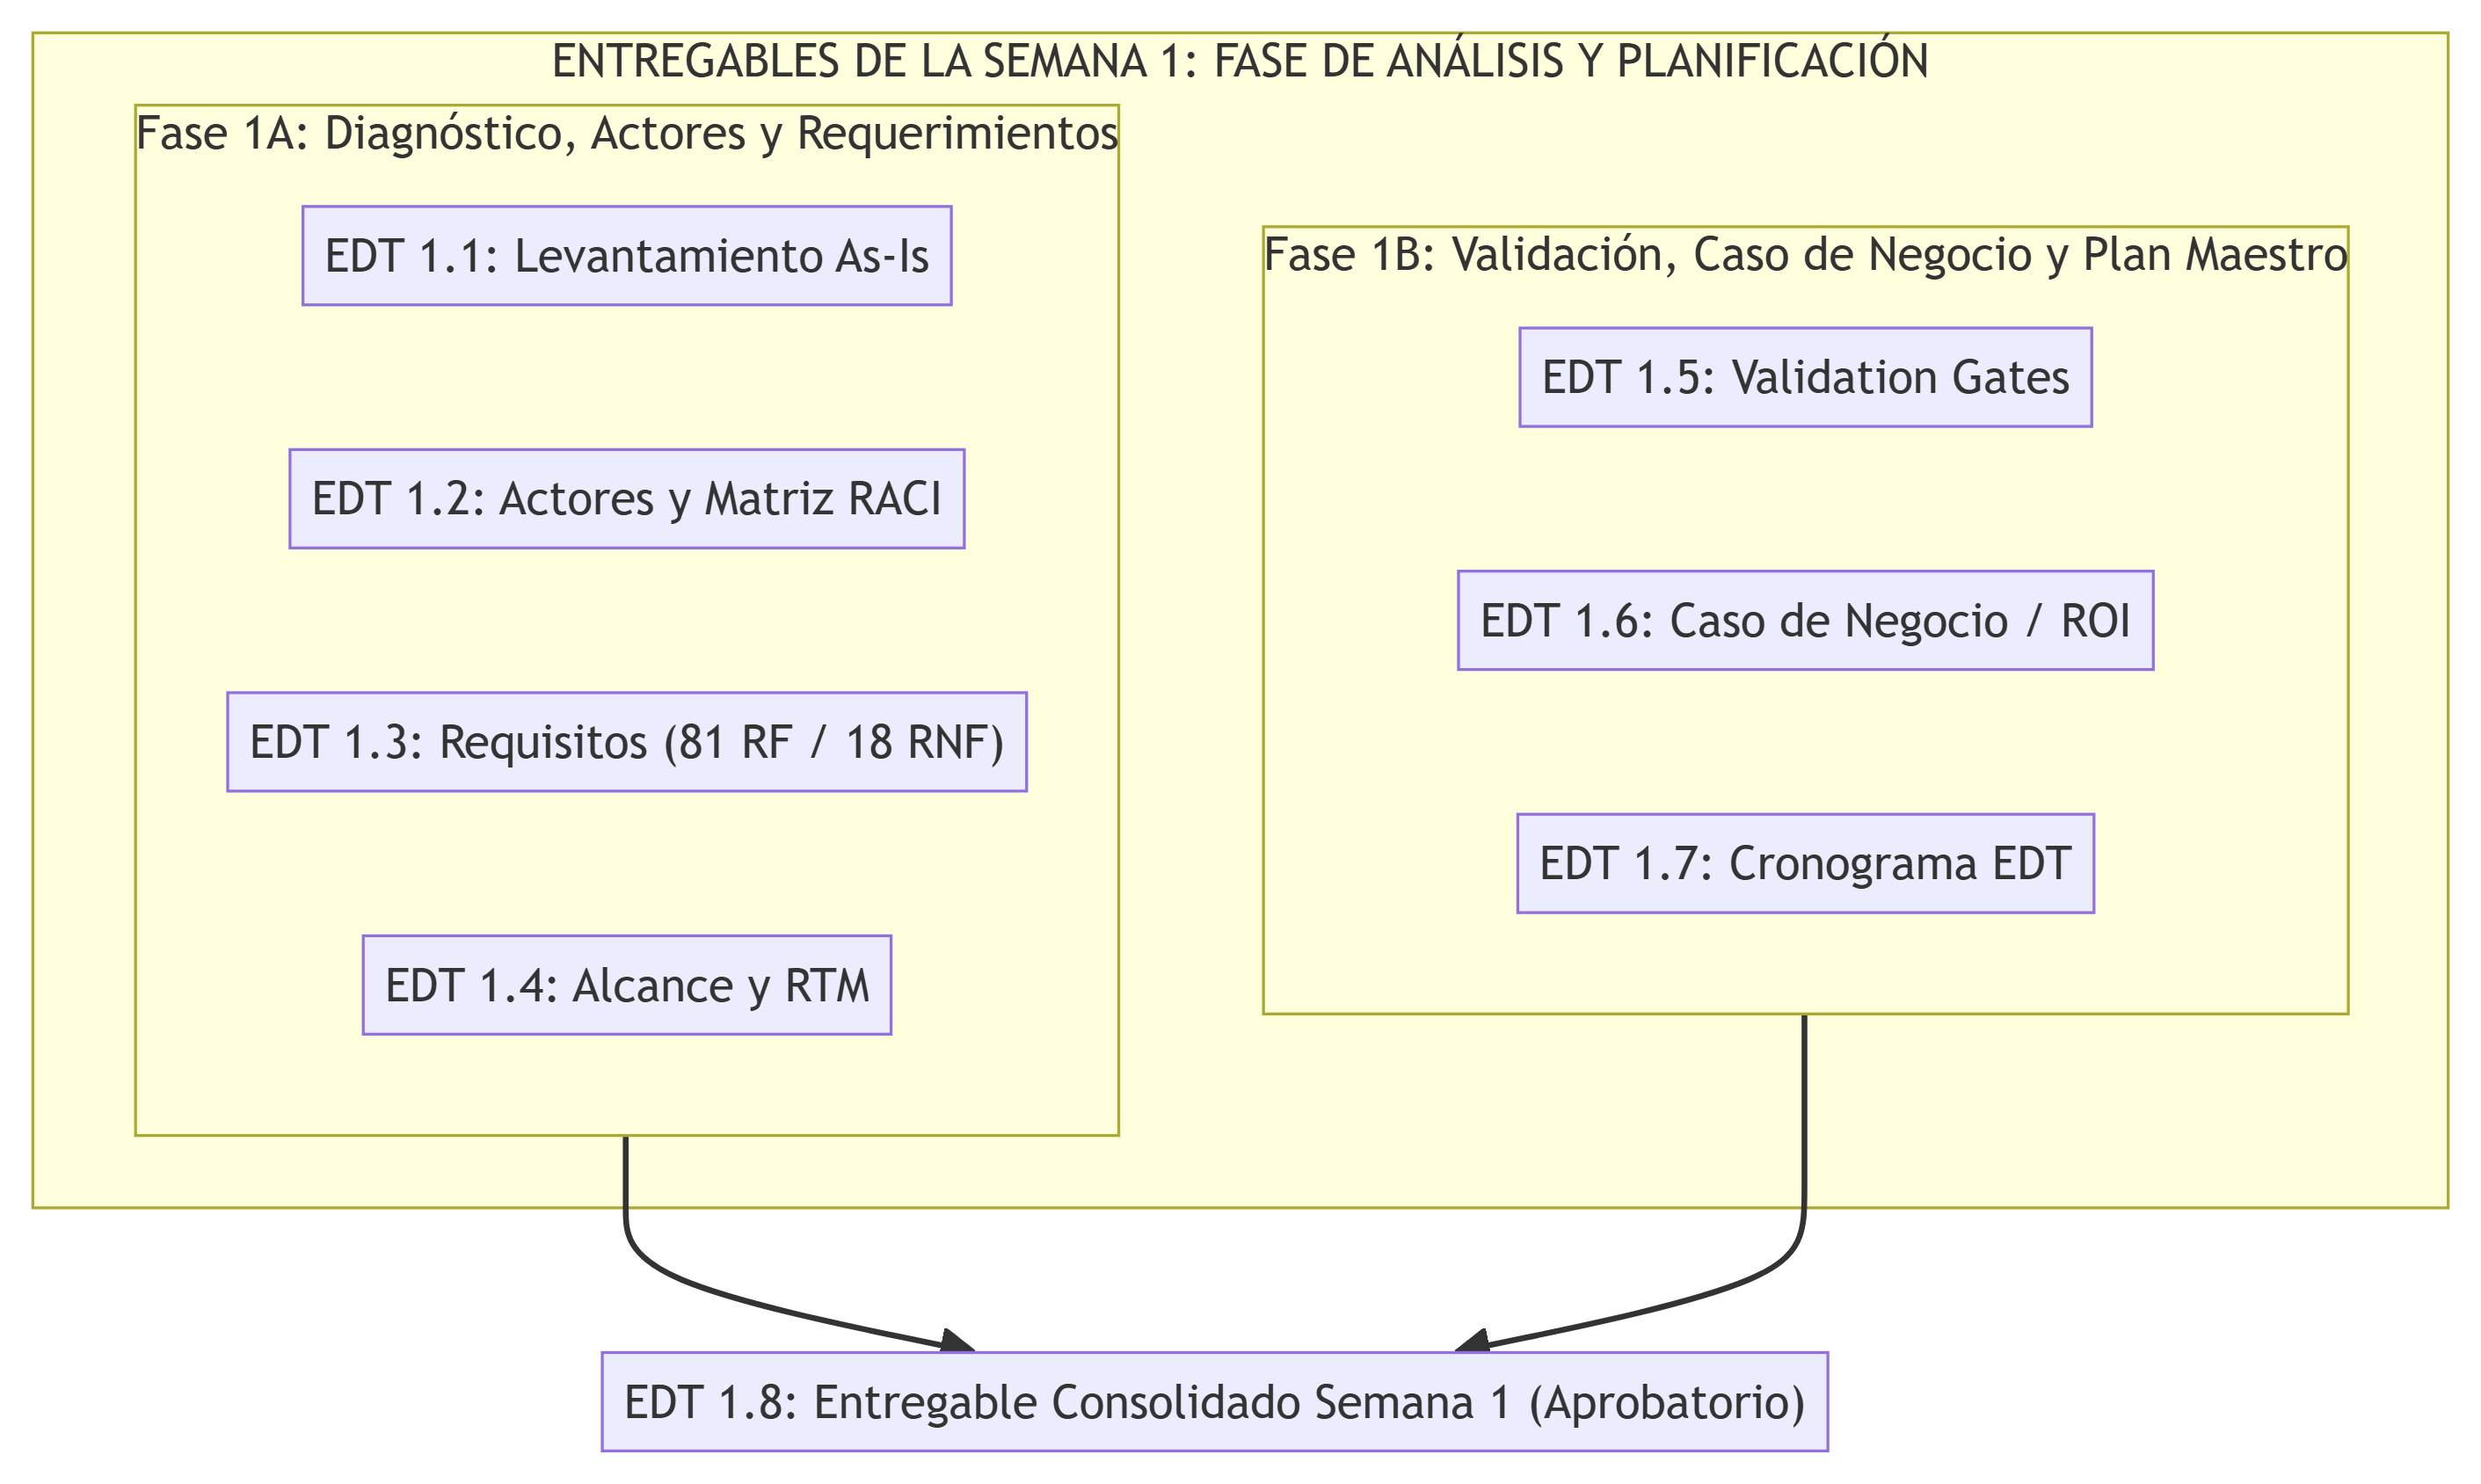
\includegraphics[width=0.88\textwidth,keepaspectratio]{images/s1_07_consolidado_s1.png}
    \caption{Mapa de Procesos y Marco Normativo de Gobernanza de Calidad en SIGE.}
    \label{fig:marco_normativo}
\end{figure}

\section{Firmas de Responsabilidad}

\noindent
\renewcommand{\arraystretch}{1.2}
\begin{tabularx}{\textwidth}{|>{\raggedright\arraybackslash}m{2.9cm}|>{\raggedright\arraybackslash}X|>{\centering\arraybackslash}m{4.6cm}|>{\centering\arraybackslash}m{2.3cm}|}
    \hline
    \rowcolor{tableheader}
    \textbf{ACCIÓN} & \textbf{NOMBRE Y CARGO} & \textbf{FIRMA} & \textbf{FECHA} \\
    \hline
    \textbf{Elaborado por:} & Heidi Villavicencio\newline Analista de Requisitos / UI-UX & \parbox[c]{4.4cm}{\centering\vspace{4pt}
\includegraphics[height=1.5cm,width=4.0cm,keepaspectratio]{images/firma_heidi.png}\vspace{4pt}} & 07/10/2026 \\
    \hline
    \textbf{Revisado por:} & Steeven Toala\newline Líder de Proyecto / Arquitecto & \parbox[c]{4.4cm}{\centering\vspace{4pt}
\includegraphics[height=1.5cm,width=4.0cm,keepaspectratio]{images/firma_steveen.png}\vspace{4pt}} & 12/10/2026 \\
    \hline
    \textbf{Aprobado por:} & Ing. Paulo Torres, Mg.\newline Docente Evaluador -- Gestión Proyectos & \parbox[c]{4.4cm}{\centering\vspace{8pt}\textbf{\textcolor{gray!80}{\scriptsize [ PENDIENTE DE APROBACIÓN ]}}\vspace{8pt}} & \textbf{\textcolor{gray!90}{Pendiente}} \\
    \hline
\end{tabularx}

\vspace{0.4cm}

\section{Control de Cambios}

\noindent
\renewcommand{\arraystretch}{1.2}
\begin{tabularx}{\textwidth}{|>{\hsize=0.45\hsize\centering\arraybackslash}X|>{\hsize=1.55\hsize\raggedright\arraybackslash}X|>{\hsize=1.2\hsize\raggedright\arraybackslash}X|>{\hsize=0.8\hsize\centering\arraybackslash}X|}
    \hline
    \rowcolor{tableheader}
    \textbf{Versión} & \textbf{Descripción del cambio} & \textbf{Responsable del cambio} & \textbf{Fecha de aprobación} \\
    \hline
    1.0 & Elaboración del Informe Técnico preliminar de normas y estándares internacionales. & Heidi Villavicencio / Steeven Toala & 07/10/2026 \\
    \hline
    2.0 & Reestructuración académica integral: priorización del núcleo normativo (ISO 25010, ISO 29148, ISO 12207, ISO 27001, IEEE 828, ISO 31000, PMBOK); reclasificación de OWASP y marcos ágiles como complementarios; exclusión justificada de CMMI e ISO 30414; incorporación del formato estándar (Qué establece, Aplicación en SIGE, Ejemplo, Evidencia) en la Sección 9; y actualización de la matriz EDT con columna de evidencia técnica. & Equipo de Desarrollo SIGE & 07/10/2026 \\
    \hline
\end{tabularx}

\vspace{0.4cm}

% =============================================================
% 12. ANEXOS
% =============================================================
\section{Anexos}

\subsection*{Anexo 1: Ficha Resumen de Familias Normativas en SIGE}
\begin{itemize}[leftmargin=1.5em, itemsep=2pt]
    \item \textbf{Normas Principales (Núcleo):} ISO/IEC 25010:2023 (Calidad del producto de software), ISO/IEC/IEEE 29148:2018 (Ingeniería de requisitos), ISO/IEC/IEEE 12207:2017 (Procesos del ciclo de vida), ISO/IEC 27001:2022 (Seguridad de la información), IEEE Std 828-2012 (Gestión de la configuración), ISO 31000:2018 (Gestión de riesgos) y PMI PMBOK 7ma Edición (Gobernanza y dirección del proyecto).
    \item \textbf{Guías Técnicas y Prácticas Complementarias:} OWASP Top 10 (Seguridad en aplicaciones web), Scrum y Kanban (Organización del trabajo del equipo), ISO 32000-1 e ISO/IEC 29500 (Formatos de intercambio documental PDF y Word).
    \item \textbf{Marcos Descartados Fundamentadamente:} CMMI (no aplicable a escala académica estudiantil) e ISO 30414 (no aplicable por ausencia de departamento formal de talento humano).
\end{itemize}

\subsection*{Anexo 2: Trazabilidad con la Estructura de Desglose del Trabajo (EDT)}
El inventario de actividades detallado en la Sección 9 guarda correspondencia unívoca con el cronograma maestro institucional registrado en el archivo \texttt{Proyecto\_SIGE\_EDT.csv} y el documento \texttt{AlcanceInforme/EDT\_Desglose\_Trabajo.md} del repositorio del proyecto SIGE.

\subsection*{Anexo 3: Declaración de Veracidad y Puntos de Verificación Pendiente}
El equipo de desarrollo declara que las descripciones del informe reflejan las actividades técnicas ejecutadas en el repositorio del proyecto. Se señalan con la etiqueta \textbf{[VERIFICAR]} aquellos aspectos que requieren comprobación empírica antes de la entrega final:
\begin{itemize}[leftmargin=1.5em, itemsep=2pt]
    \item \textbf{Verificación 1 (Pruebas de Carga Concurrente):} Comprobar si el equipo ejecutó la simulación de concurrencia con herramientas como Apache JMeter o k6, o si se mantiene como criterio de aceptación para la fase de pruebas de estrés.
    \item \textbf{Verificación 2 (Límites WIP en Trello):} Confirmar si el tablero Trello operó con límites WIP numéricos configurados o si se utilizó como panel de seguimiento visual de estados.
\end{itemize}

\end{document}
